\documentclass[14pt]{beamer}
\mode<presentation>
%\graphicspath{{image/}}
\usepackage{listings}
\usepackage{verbatim}

\usecolortheme{whale}
\usecolortheme{orchid}
\useinnertheme{rounded}
\useinnertheme{circles}
\setbeamertemplate{headline}[default]


\title{IWI Programmeerwedstrijd 2010\\\vspace{4mm}\normalsize{}The Results}
\author{}
\date{2010-05-22}

\begin{document}

%======================================================================================

%--------------------------------------------------------------------------------------
\frame{\titlepage}
%--------------------------------------------------------------------------------------

%======================================================================================
\section{Resultaten}
\subsection{}
%======================================================================================

\begin{frame}
  \frametitle{Statistics}
  \begin{tabular}{ll}
    Eerste goede inzending: & 13 minuten\\
    Laatste inzending       & 16 seconden voor einde \\
    Laatste goede inzending & 7 minuten voor einde \\
    Number of submissions:  & 78 $\approx$ 10 per team,\\& 2.6 correct\\
  \end{tabular}
\end{frame}

\begin{frame}
  \frametitle{Results}
  \begin{block}{Zwaar}
    \begin{enumerate}
     \vspace*{7mm}
     \item<4->          \Large      Team TEEM \textit{(6.5)}
     \vspace*{5mm}
     \item<3->          \large      Team[0] \textit{(4, 669 min.)}
     \vspace*{5mm}
     \item<2->          \normalsize Team Awesome!!!\~{}$|$1! \textit{(4, 729 min.)}
     \vspace*{7mm}
    \end{enumerate}
  \end{block}
\end{frame}

%======================================================================================
\section{Problems}
%\subsection{}
%======================================================================================

\begin{frame}
  \frametitle{Problems}
  \begin{center}
    \Huge{FAIL}
  \end{center}
\end{frame}

\begin{frame}[fragile]
  \frametitle{Problems}
  \begin{block}{drumstick != kip}
\small
\begin{lstlisting}[language=C++]
void run() {
    int nChickens = in.nextInt();
    System.out.println(nChickens/5);
}
\end{lstlisting}
  \end{block}
\end{frame}


\begin{frame}[fragile]
  \frametitle{Problems}
  \begin{block}{Angle of a vector}
\tiny
\vspace*{-5mm}\hspace*{-10mm}\begin{lstlisting}[language=C++]
if (x== 0 && y > 0) {
    angle = 0.0;
} else if (x== 0) {
    angle = 180.0;
} else if (y == 0 && x> 0) {
    angle = 90.0;
} else if (y == 0) {
    angle = 270.0;
} else {
    if (x< 0 ^ y < 0) {
        angle = Math.toDegrees(Math.atan(Math.abs((double)y/(double)rodsX[i])));
    } else {
        angle = Math.toDegrees(Math.atan(Math.abs((double)rodsX[i]/(double)y)));
    }
    if (x< 0 && y < 0) {
        angle += 180;
    } else if (x< 0) {
        angle += 270;
    } else if (y < 0) {
        angle += 90;
    }
}
\end{lstlisting}
  \end{block}
\end{frame}
\begin{frame}[fragile]
  \frametitle{Problems}
  \begin{block}{Angle of a vector}
\begin{lstlisting}[language=C++]
angle = Math.atan2(y,x);
\end{lstlisting}
  \end{block}
\end{frame}


%-----------------------------------------------------
% Van makkelijk naar moeilijk

\begin{frame}
  \frametitle{Opgaven}
  \begin{center}
    \Huge{De antwoorden}
  \end{center}
\end{frame}

\subsection{A. The Morning Train}
\begin{frame}
  \frametitle{A. The Morning Train}
    \large
    \begin{itemize}
      \vspace*{-2mm}
      \item Simulatie.
            Priority queue met ticket machines.
      \vspace*{5mm}
      \item Een array werkt ook, want er zijn maximaal 9.
      \vspace*{5mm}
      \item Eerst tickets, dan poortjes.
    \end{itemize}
\end{frame}

\subsection{B. Forklift}
\begin{frame}
  \frametitle{B. Forklift}
      \only<1>{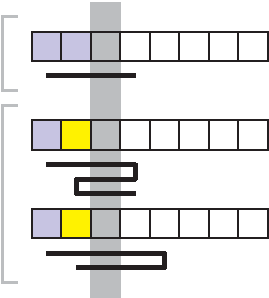
\includegraphics[width=65mm]{forklift}}%
\end{frame}

\subsection{C. Tiltmaze}
\begin{frame}
  \frametitle{C. Tiltmaze}
    \large
    \begin{itemize}
      \vspace*{-2mm}
      \item Breadth-first search
      %\vspace*{5mm}
      %\item BLA
    \end{itemize}
\end{frame}

\subsection{D. Downhill}
\begin{frame}
  \frametitle{D. Downhill}
  \only<1>{
    \large
    \begin{itemize}
      \vspace*{-2mm}
      \item Moet in $\mathcal{O}(n\log n)$
    \end{itemize}
  }%
    \centering%
      \only<2>{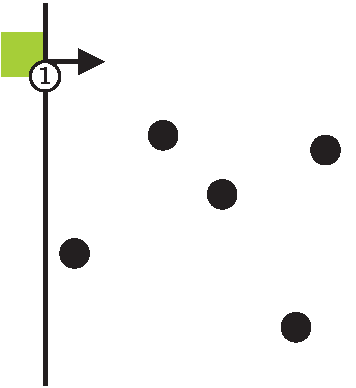
\includegraphics[width=6cm]{downhill1}}%
      \only<3>{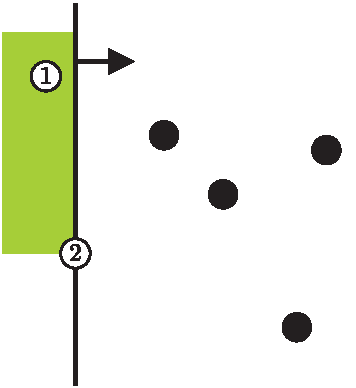
\includegraphics[width=6cm]{downhill2}}%
      \only<4>{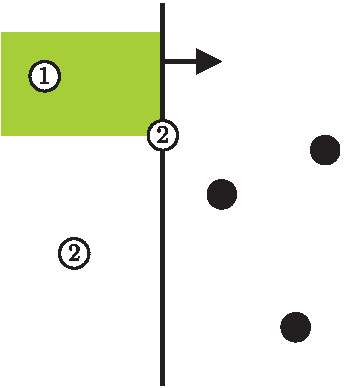
\includegraphics[width=6cm]{downhill3}}%
      \only<5>{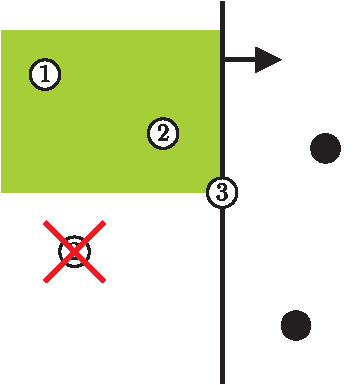
\includegraphics[width=6cm]{downhill4}}%
      \only<6>{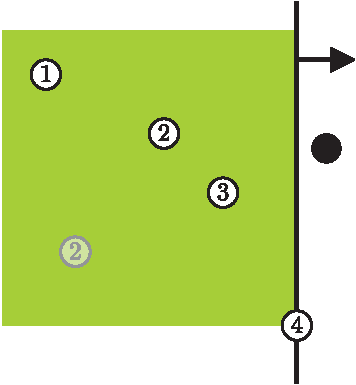
\includegraphics[width=6cm]{downhill5}}%
      \only<7>{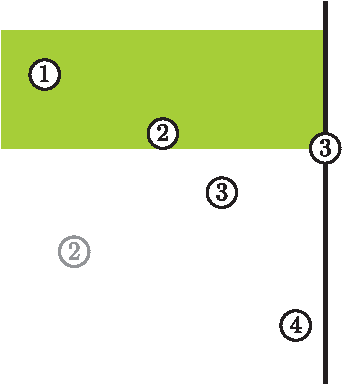
\includegraphics[width=6cm]{downhill6}}%
\end{frame}

\subsection{E. Dining Philosophers}
\begin{frame}
  \frametitle{E. Dining Philosophers}
    \large
    \begin{itemize}
      \vspace*{-2mm}
      \item $\text{input}/5$
    \end{itemize}
\end{frame}

\subsection{F. Settle the Bill}
\begin{frame}
  \frametitle{F. Settle the Bill}
    \large
    \begin{itemize}
      \vspace*{-2mm}
      \item In een subset met som 0, betalen in een kring.
      \vspace*{5mm}
      \item<2-> Kan met $n-1$ betalingen.
      \vspace*{5mm}
      \item<2-> Is er een niet lege stricte subset met som 0?
      % kan niet anders??
    \end{itemize}
\end{frame}

\subsection{G. Detector Dodging}
\begin{frame}
  \frametitle{G. Detector Dodging}
    \large
    \begin{itemize}
      \vspace*{-2mm}
      \item Hoeken sorteren.
      \vspace*{5mm}
      \item Houd rekening met de laatste.
    \end{itemize}
\end{frame}

\subsection{H. Java Decompiler}
\begin{frame}
  \frametitle{H. Java Decompiler}
    \large
    \begin{itemize}
      \vspace*{-2mm}
      \item Haakjes!
      \vspace*{5mm}
      \item Sorry voor de fout in het voorbeeld.
    \end{itemize}
\end{frame}

\subsection{I. Compression}
\begin{frame}
  \frametitle{I. Compression}
    \large
    \begin{itemize}
      \vspace*{-2mm}
      \item Je bent volledig vrij!
      \vspace*{5mm}
      \item Hier zijn wat ideeen:
            \begin{tabular}{ll}
            CamelCase                 & 87\% \\
            woorden vervangen         & 82\% \\
            ngrams + Huffman + base64 & 65\% \\
            maak woordenboek          & 50\% \\
            \end{tabular}
    \end{itemize}
\end{frame}
\begin{frame}[fragile]
  \frametitle{I. Compression}
  \footnotesize
\begin{lstlisting}[language=C++]
class P {
    public static void Main(string[] args) {
        Console.ReadLine();
        Console.WriteLine(Console.ReadLine()
                         .Replace("qu","_")
                         .Replace("q","qu")
                         .Replace("_","q"));
    }
}
\end{lstlisting}
\end{frame}



%======================================================================================
\section{Tot volgend jaar!}
%\subsection{}
%======================================================================================

\begin{frame}
  \frametitle{Tot volgend jaar!}
  \begin{block}{Pizza@}
    Pizzeria Rigoletto\\
    Nieuwe Ebbingestraat\\
    19:00
  \end{block}
\end{frame}

\end{document}
